\documentclass[11pt]{beamer}
\usetheme{Warsaw}
\usepackage[utf8]{inputenc}
\usepackage[russian]{babel}
\usepackage[OT1]{fontenc}
\usepackage{amsmath}
\usepackage{amsfonts}
\usepackage{amssymb}
\usepackage{graphicx}
\usepackage{listings}
%\author{Albert}
\title{Эффективная работа с процедурными деревьями}
%\setbeamercovered{transparent} 
%\setbeamertemplate{navigation symbols}{} 
%\logo{} 
%\institute{} 
%\date{} 
%\subject{} 
\begin{document}

\begin{frame}
\titlepage
\end{frame}

%\begin{frame}
%\tableofcontents
%\end{frame}

\begin{frame}{Процедурная генерация в играх}
На данный момент существует множество разнообразных алгоритмов
для процедурной генерации в играх или для визуализации.
Также есть проекты, позволяющие создавать реалистичные модели
деревьев с высокой детализацией.
Например, SpeedTree: %ссылка
%картинка дерева оттуда
\begin{figure}[hbtp]
\centering
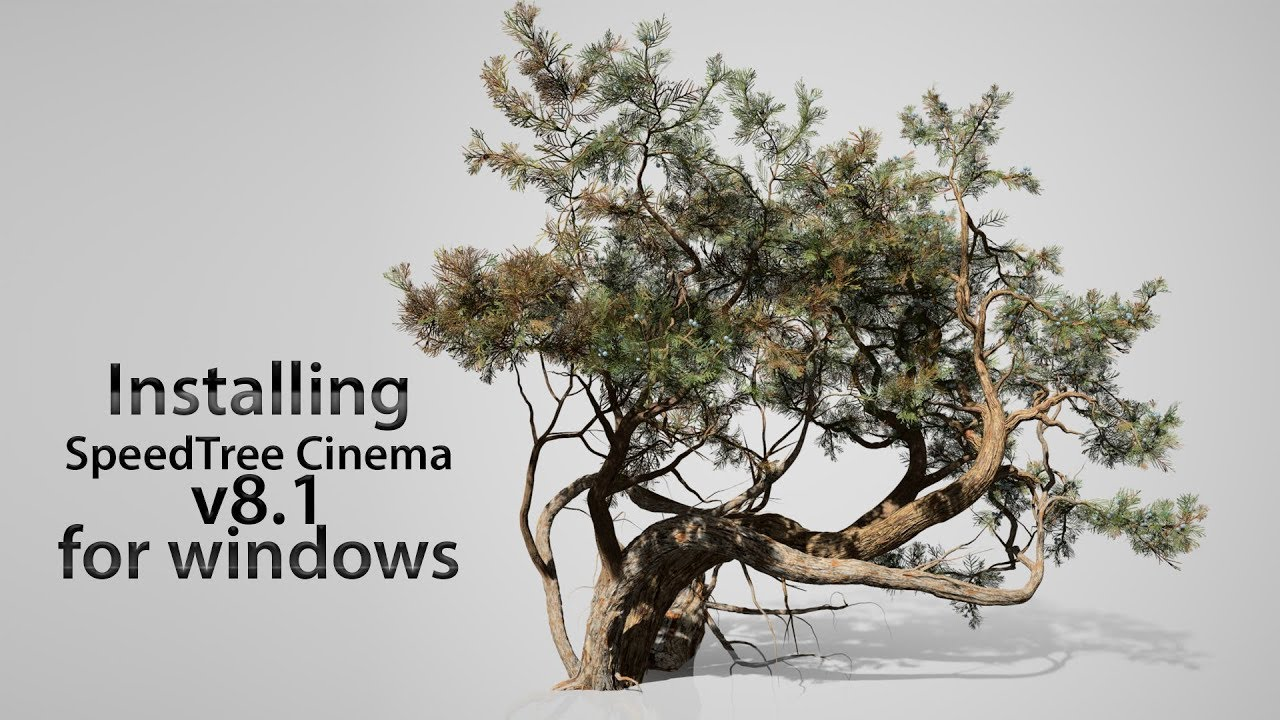
\includegraphics[scale=0.2]{st.jpg}
\end{figure}
\end{frame}
\begin{frame}{Преимущества}
- Огромные открытые миры\linebreak
- Генерация по мере игры\linebreak
- Внешнее разнообразие\linebreak
- Уникальный игровой опыт\linebreak
- Меньше работы художников, дизайнеров уровней\linebreak
- Зависимость от окружения
%процедурные деревья, образующие лес, могут выглядеть естественно
%если их генерация учитывала их взаимодействие друг с другом, освещенность
% и т.д. Вручную достичь этого куда сложнее
\end{frame}
\begin{frame}{Проблемы и ограничения}
- у человека часто получается лучше\linebreak
- не подходит для точно выверенного level-дизайна\linebreak\linebreak
%так в Dota2 на карте все деревья расставлены со смыслом
%их точное расположение важно, тк можно прятаться, устраивать засады
основная проблема:\linebreak
\textbf{   Слишком много уникальных моделей   }

\end{frame}
\begin{frame}{Что делать?}
- использование заранее подготовленного набора моделей (обычно)\linebreak
%в таком случае процедурная генерация сводится к расстановке их по карте
%некоторым простым трансформациям и т.д.
%большинство игр с процедурно генерируемым миром поступает именно так
- создание моделей "на лету"\ (не всегда подходит)\linebreak
%такой подход часто используется для совсем простых структур типа травы
%но если требуется сложная геометрия, то так врядли получится
- создание моделей из стандартных элементов (Minecraft)\linebreak
%пример такого подхода - майнкрафт, где деревья и прочие структуры игрового мира состоят из блоков нескольких типов
\end{frame}
\begin{frame}{Развиваем третий подход}
%переходим к основной части презентации 
\textbf{"Сборные"\ деревья}\linebreak
или\linebreak
уникальность и эффективность одновременно
\end{frame}
\begin{frame}{General pipeline}
%здесь диаграмма
\begin{figure}[hbtp]
\centering
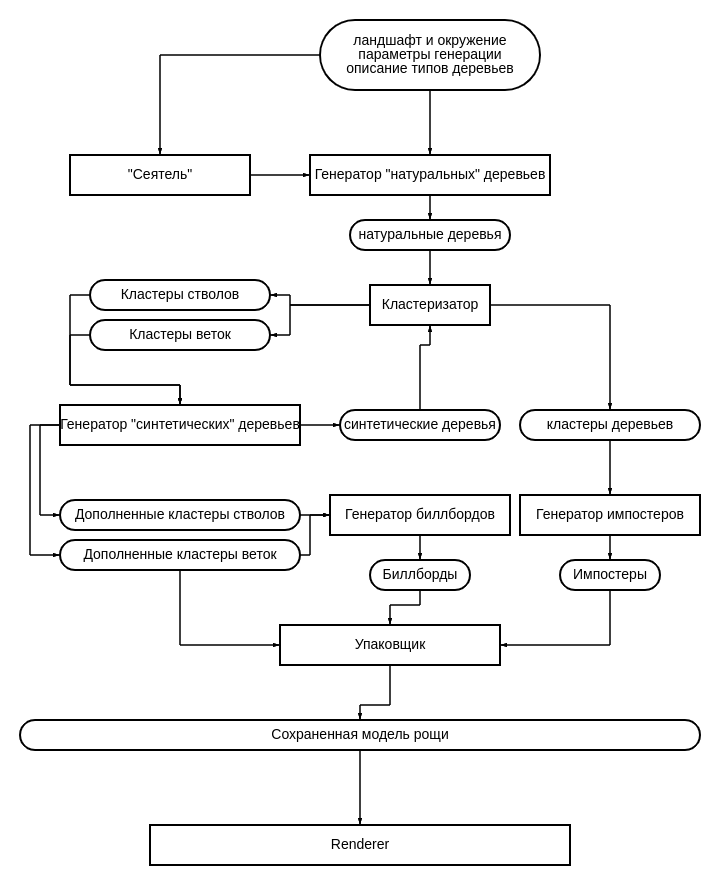
\includegraphics[scale=0.25]{diagram.png}
\end{figure}
\end{frame}
\begin{frame}{Генератор натуральных деревьев}
Основная задача - создание группы деревьев с учетом переданных параметров
и свойств окружающей среды.\linebreak\linebreak
Входные параметры:\linebreak
 - карта высот и "пригодности" для роста\linebreak
 - описание типов деревьев  \linebreak
 - объекты на сцене - например, Bounding Boxes для геометрии уровня\linebreak
 - общие параметра генератора (количество деревьев, точность генерации)\linebreak

\end{frame}
\begin{frame}{Посадить дерево}
Генератор работает итеративно - на каждом шаге возможна посадка новых деревьев и рост уже существующих. \linebreak
Для выбора места посадки поддерживается карта пригодности:\linebreak

$hab(x,y) = \frac{A}{1 + shade(x,y)}*mask(x,y)*(B*f(h(x,y)) + BH(x,y))$ 
$f(h(x,y)) = M - grad(h)(x,y)$
\linebreak\linebreak Shade - карта уровня затененности на плоскости - каждый узел и лист дерева увеличивает затененность там, где он находится.
\end{frame}
\begin{frame}{Вырастить дерево}
Дерево представляется иерархической структурой веток, состоящих из вершин и сегментов, из вершин растут дочерние ветки\linebreak 
Процесс итеративный, основан на распределении питательных веществ по дереву и их конвертацию в рост новых веток, удлинение или продление текущих\linebreak \linebreak 
На каждой итерации\linebreak 
- считаем освещенность в каждом листе и аккумулируем в корне\linebreak 
- распределяем из корня питательные вещества иерархически по веткам, отдавая предпочтение тем вершинам, из которых можно что-то вырастить
- пытаетмся вырастить новые ветки или сегменты\linebreak 
- пересчитываем толщину веток\linebreak 
\end{frame}
\begin{frame}{Вырастить дерево}
\begin{figure}[hbtp]
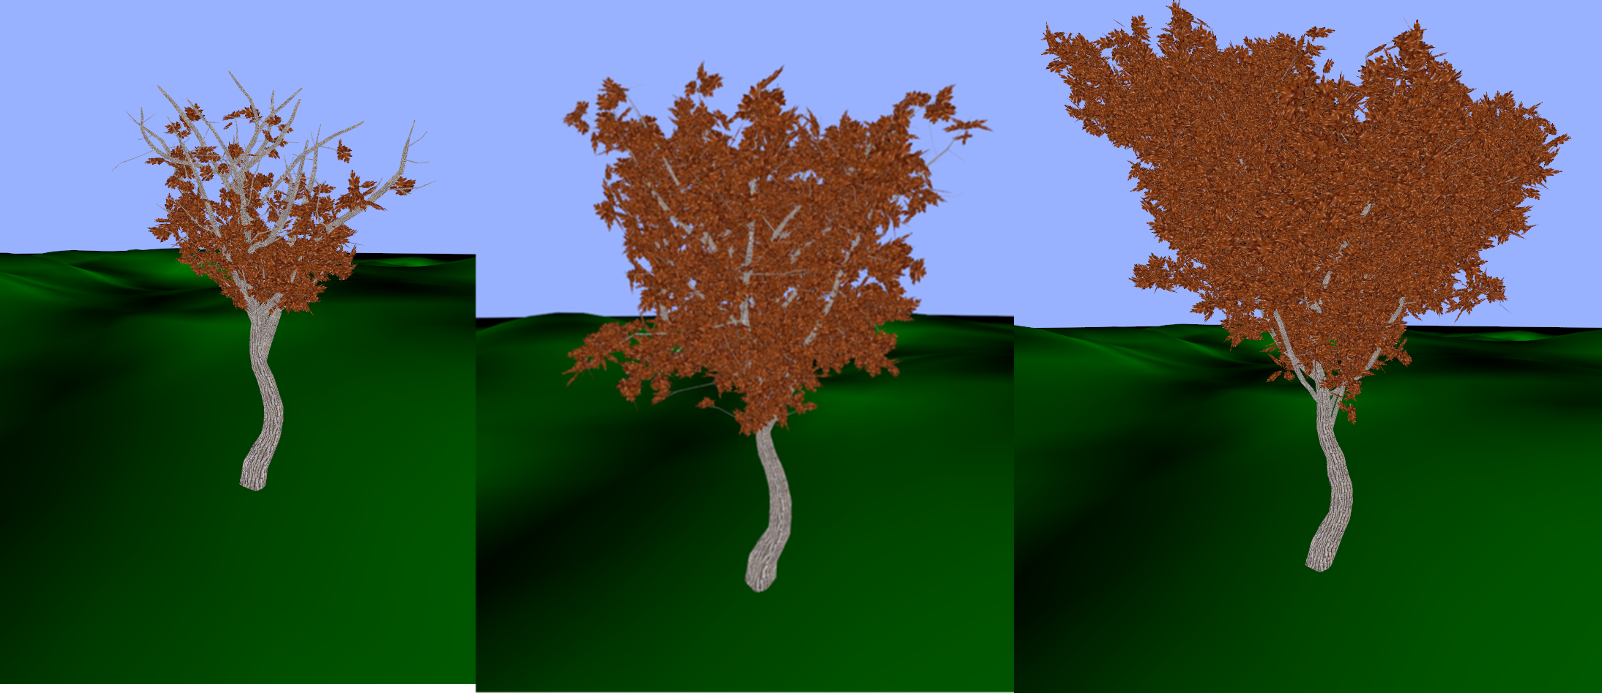
\includegraphics[scale=0.2]{iterations.png}
\caption{25, 100, 1000 итераций роста}
\end{figure}
\end{frame}
\begin{frame}{Распределение питательных веществ}
\begin{figure}[hbtp]
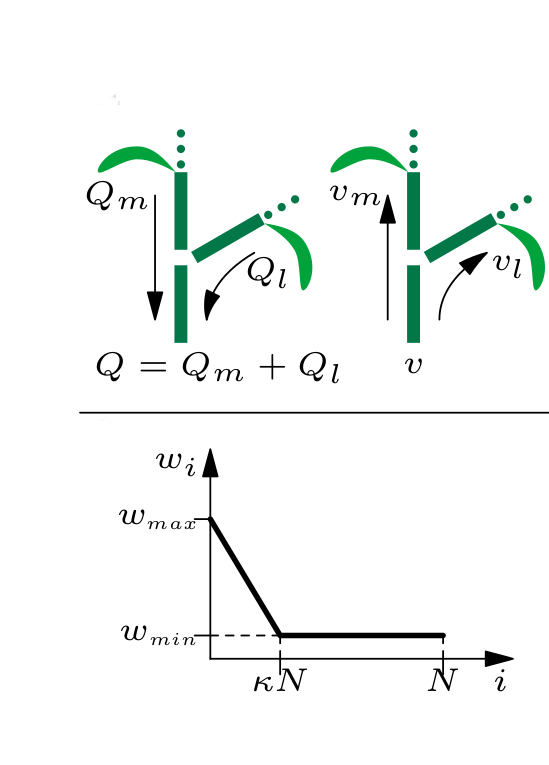
\includegraphics[scale=0.3]{weights.png}
\end{figure}
\end{frame}
\begin{frame}{Воксельная карта освещения}
\begin{figure}[hbtp]
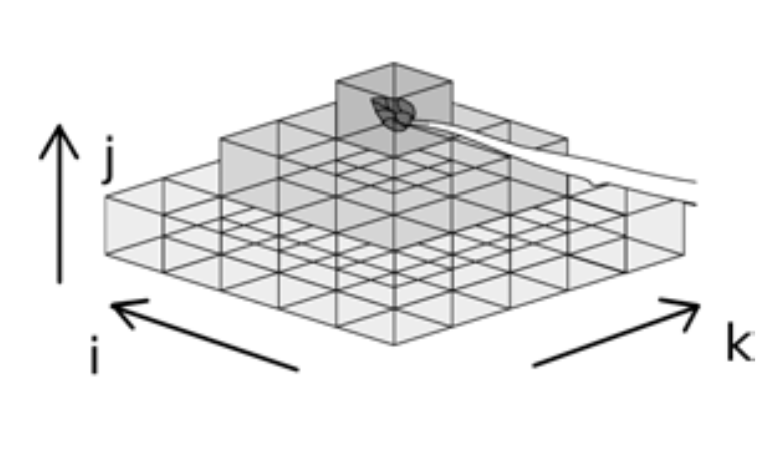
\includegraphics[scale=0.4]{shadow.png}
\end{figure}
\end{frame}
\begin{frame}{Воксельная карта освещения}
\begin{figure}[hbtp]
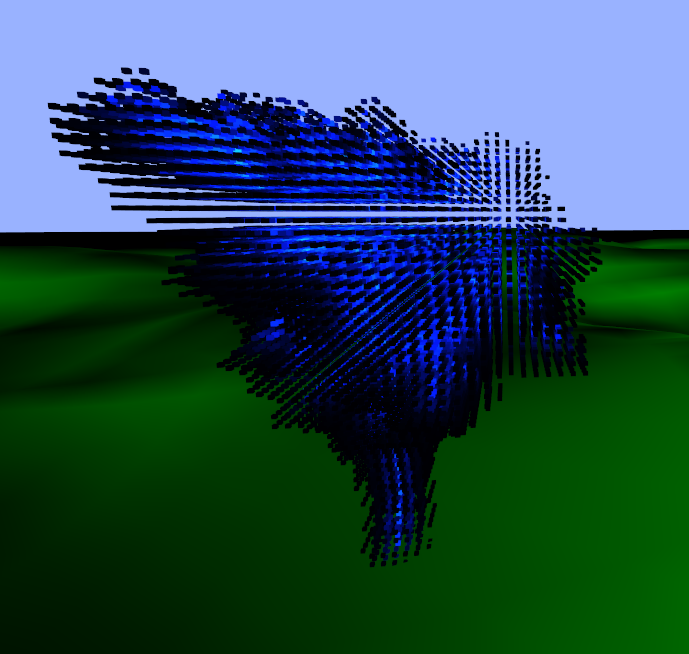
\includegraphics[scale=0.3]{voxels.png}
\caption{Воксельная тень от дерева}
\end{figure}
\end{frame}
\begin{frame}{Направление роста}
- В окрестности вершины определяется направление с максимальной освещенностью и уровень освещенности\linebreak 
- Для небольших веток - это минимум по соседним вокселям, для более крупных применяется трассировка конусами\linebreak 
- Соотношение уровня освещенности и количества питательных веществ определяет вероятность роста новой ветки\linebreak 
- На ее направление также влияют постоянные параметра дерева и ее положение в структуре дерева\linebreak 
\end{frame}
\begin{frame}{Параметры}
\begin{figure}[hbtp]
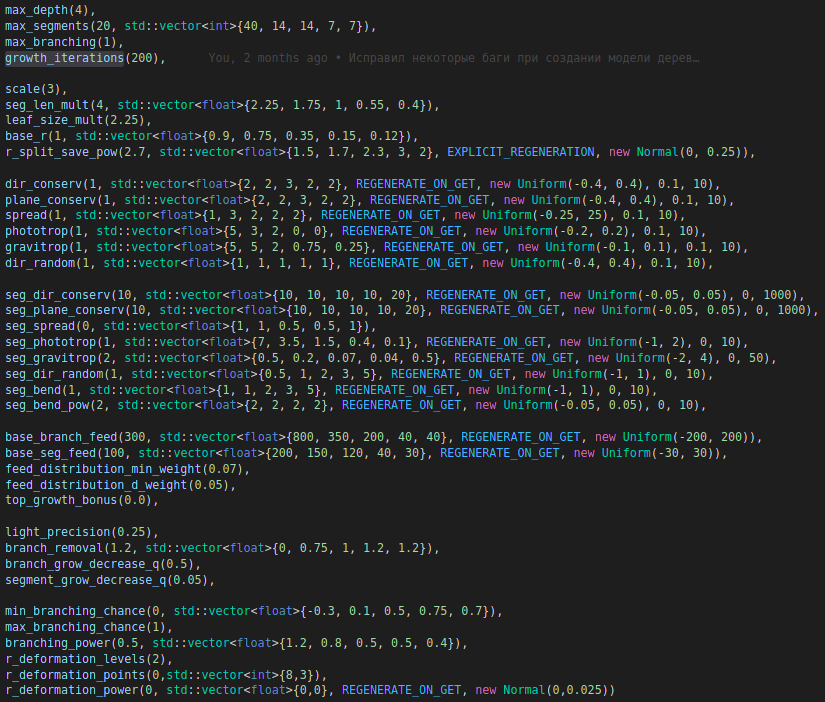
\includegraphics[scale=0.275]{parameters.png}
\caption{Список параметров генератора}
\end{figure}
\end{frame}
\begin{frame}{Разнообразие}
\begin{figure}[hbtp]
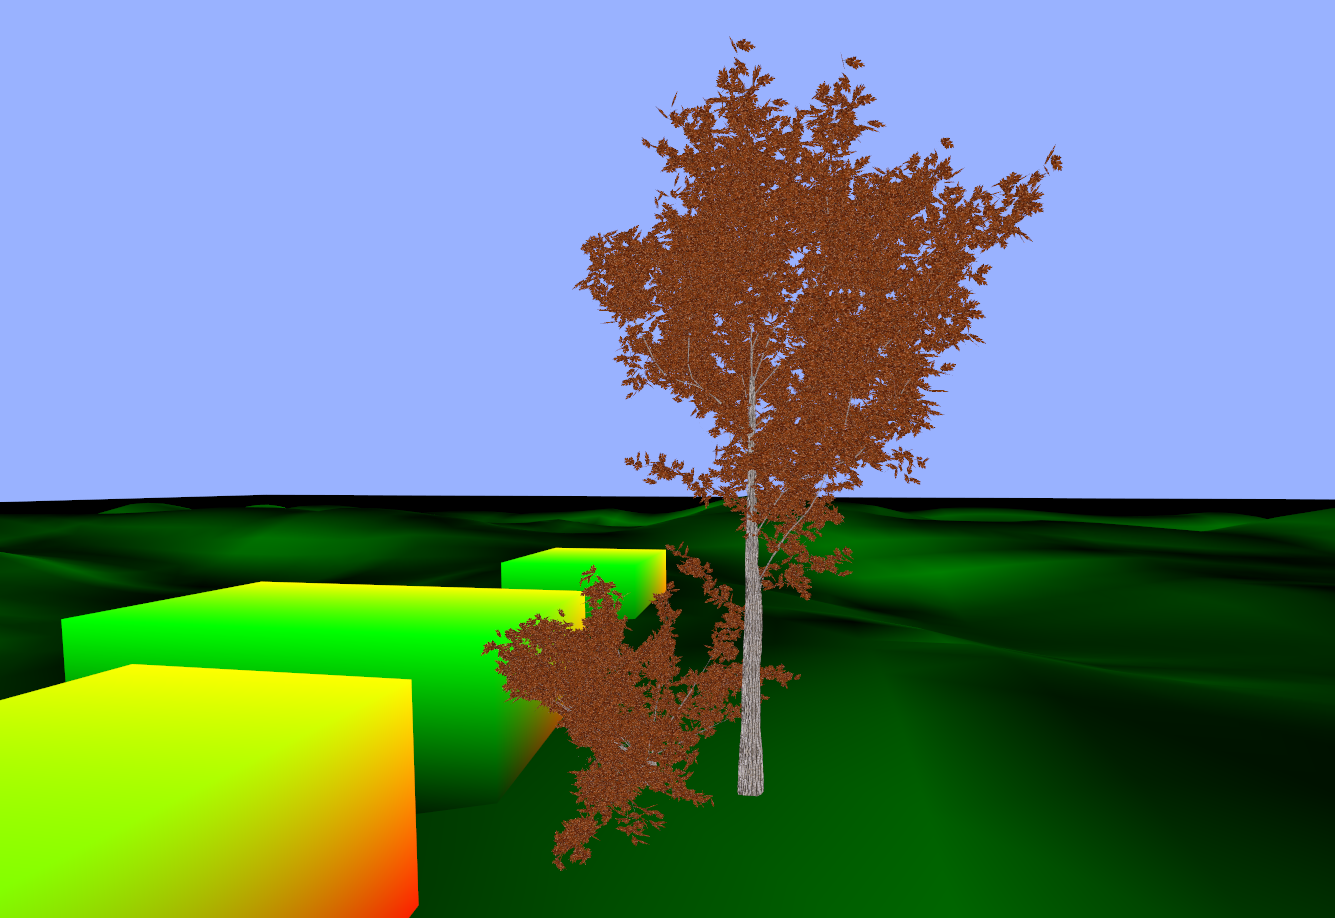
\includegraphics[scale=0.215]{div.png}
\caption{Различные наборы параметров позволяют создавать растения разных форм и размеров}
\end{figure}
\end{frame}
\begin{frame}{Кластеризация}

\textbf{Задача}:\linebreak По множеству уникальных деревьев построить набор базовых структурных элементов, из которых, используя простые геометрические преобразования, можно получить деревья, внешне минимально отличающиеся от исходных.
\end{frame}
\begin{frame}{Кластеризация}
Представим дерево как ствол и множество веток, растущих непосредственно из него. \linebreak
Соберем стволы и ветки всех деревьев вместе и разделим на группы (кластеры) похожих.\linebreak
Сохраним по одному представителю каждого кластера, а остальных выразим через него с помощью матриц трансформации.
\end{frame}
\begin{frame}{Кластеризация}
Зная метрику расстояния между любыми двумя элементами множества, мы можем
разделить его на кластеры одним из существующих общих алгоритмов 
\begin{figure}[hbtp]
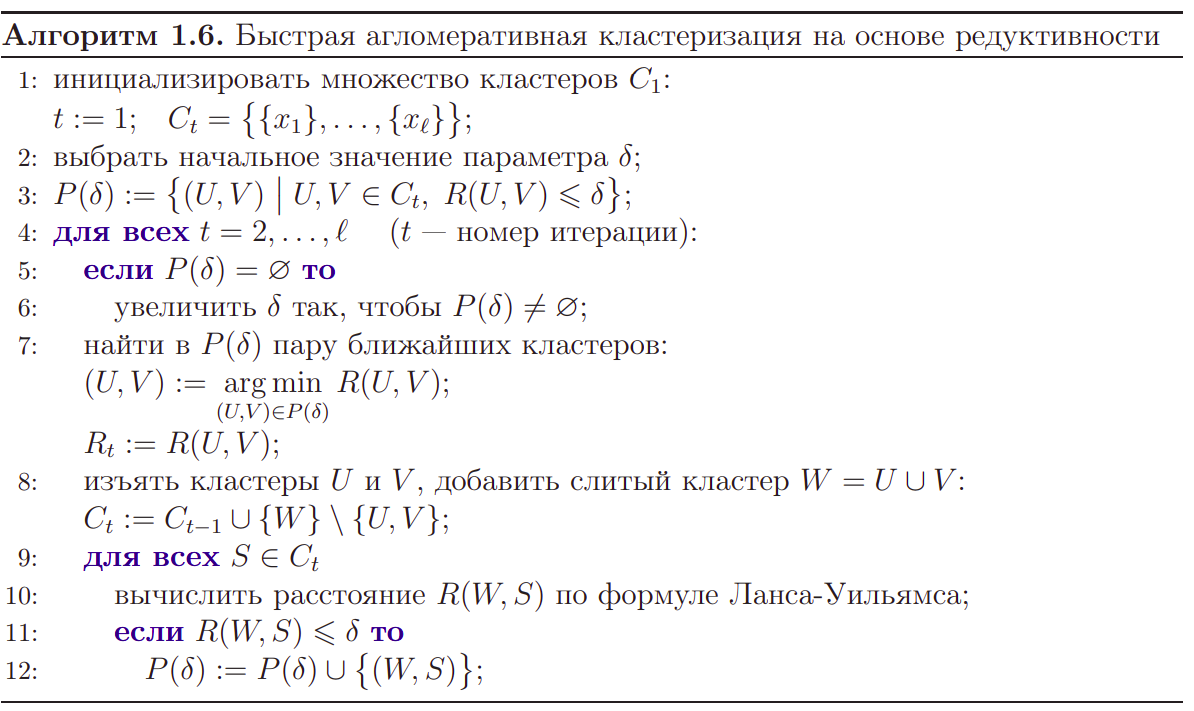
\includegraphics[scale=0.225]{c1.png}
\end{figure}
\end{frame}
\begin{frame}{Кластеризация}
\begin{figure}[hbtp]
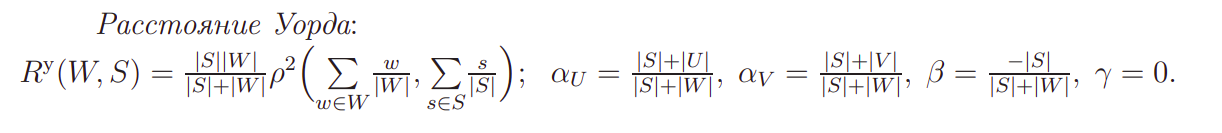
\includegraphics[scale=0.275]{c2.png}
\end{figure}
формула Ланса-Уильямса:
\begin{figure}[hbtp]
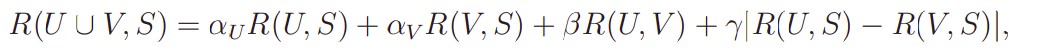
\includegraphics[scale=0.275]{c3.png}
\end{figure}
\end{frame}
\begin{frame}{Оптимизации}
- все результаты вычисления индивидуальных расстояний кэшируются\linebreak 
- есть предел на индивидуальную дистанцию между двумя элементами кластера\linebreak 
- функция расстояния завершает работу, если предельное расстояние достигнуто\linebreak 
\end{frame}
\begin{frame}{Метрика расстояния ("похожести")}
Все ветки нормализуются - трансформируются так, чтобы их 
Bounding box был единичным кубом\linebreak 
Метрика расстояния:\linebreak \linebreak 
$M(B_1,B_2) = \min_{\alpha \in [0,2\pi]} M_0(B_1,rotate(B_2,\vec{x},\alpha))$
$M_0 = a*M_{struct}*(1 - b*R_{diff}) + (1 - a)*M_{light}$

$M_{struct}$ - метрика структурной "похожести"\linebreak 
$M_{light}$ - метрика "похожести" затенения\linebreak 
$R_{diff}$ - показатель разницы в толщине веток\linebreak 


\end{frame}
\begin{frame}{Метрика структурной "похожести"}
- Сопоставляем вершины сравниваем веток друг с другом\linebreak 
- Начинаем с вершин собственно самих веток, сопоставлению подлежат вершины, находящиеся на расстоянии не более $\delta*len$, где 
$\delta$ - заданная константа\linebreak 
$len$ - длина кратчайшей из сравнивемых веток\linebreak 
- Рекурсивно проводим процедуру сопоставления для дочерних веток, растущих из сопоставленных вершин\linebreak 
Формально получаем множество пар:\linebreak $MJ = \{(j_1,j_2), j_1 \in B_1, j_2 \in B_2\}$
\linebreakТогда:\linebreak\linebreak
$M_{struct} = \frac{1}{W_s}*\frac{\sum_{(j_1,j_2) \in MJ} (sw(j_1.level) + sw(j_2.level))}{\sum_{j_1 \in B_1} sw(j_1.level) + \sum_{j_2 \in B_2} sw(j_2.level)}$\linebreak
$sw(n)$ - константный массив весов для возможных уровней вершин\linebreak
$W_s$ - нормировочный множитель
\end{frame}
\begin{frame}{Метрика структурной "похожести"}
\[R_{diff} = \frac{1}{W_r}*(\sum_{(j_1,j_2) \in MJ} \int_{0}^{2\pi} \frac{|j_1.r(\alpha) - j_2.r(\alpha)|}{|j_1.r(\alpha) + j_2.r(\alpha)|} \,d\alpha)\]\linebreak
$W_r$ - нормировочный множитель
\[M_{light} = \iiint_V \frac{|V_1(x,y,z) - V_2(x,y,z)|}{V_1(x,y,z) + V_2(x,y,z)} \,dx\,dy\,dz\]
\end{frame}
\begin{frame}{Без кластеризации}
\begin{figure}[hbtp]
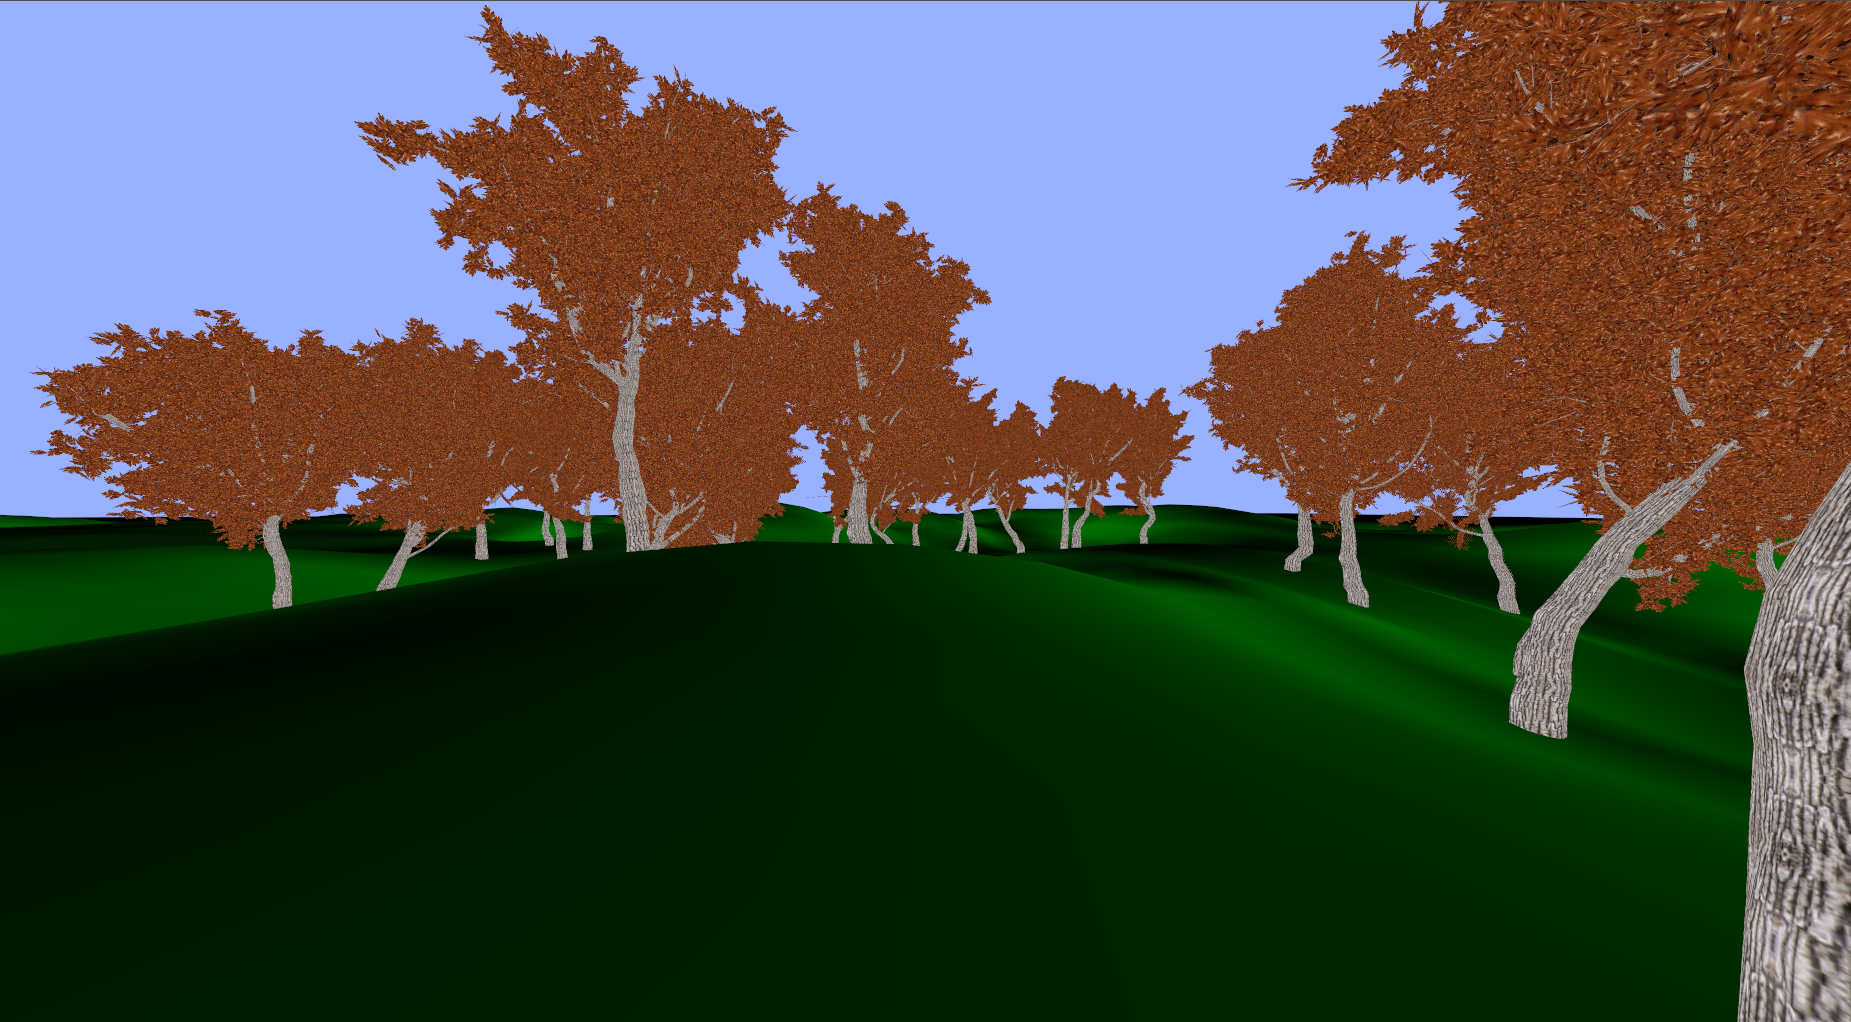
\includegraphics[scale=0.18]{no_clust.png}
\end{figure}
\end{frame}
\begin{frame}{С кластеризацей}
\begin{figure}[hbtp]
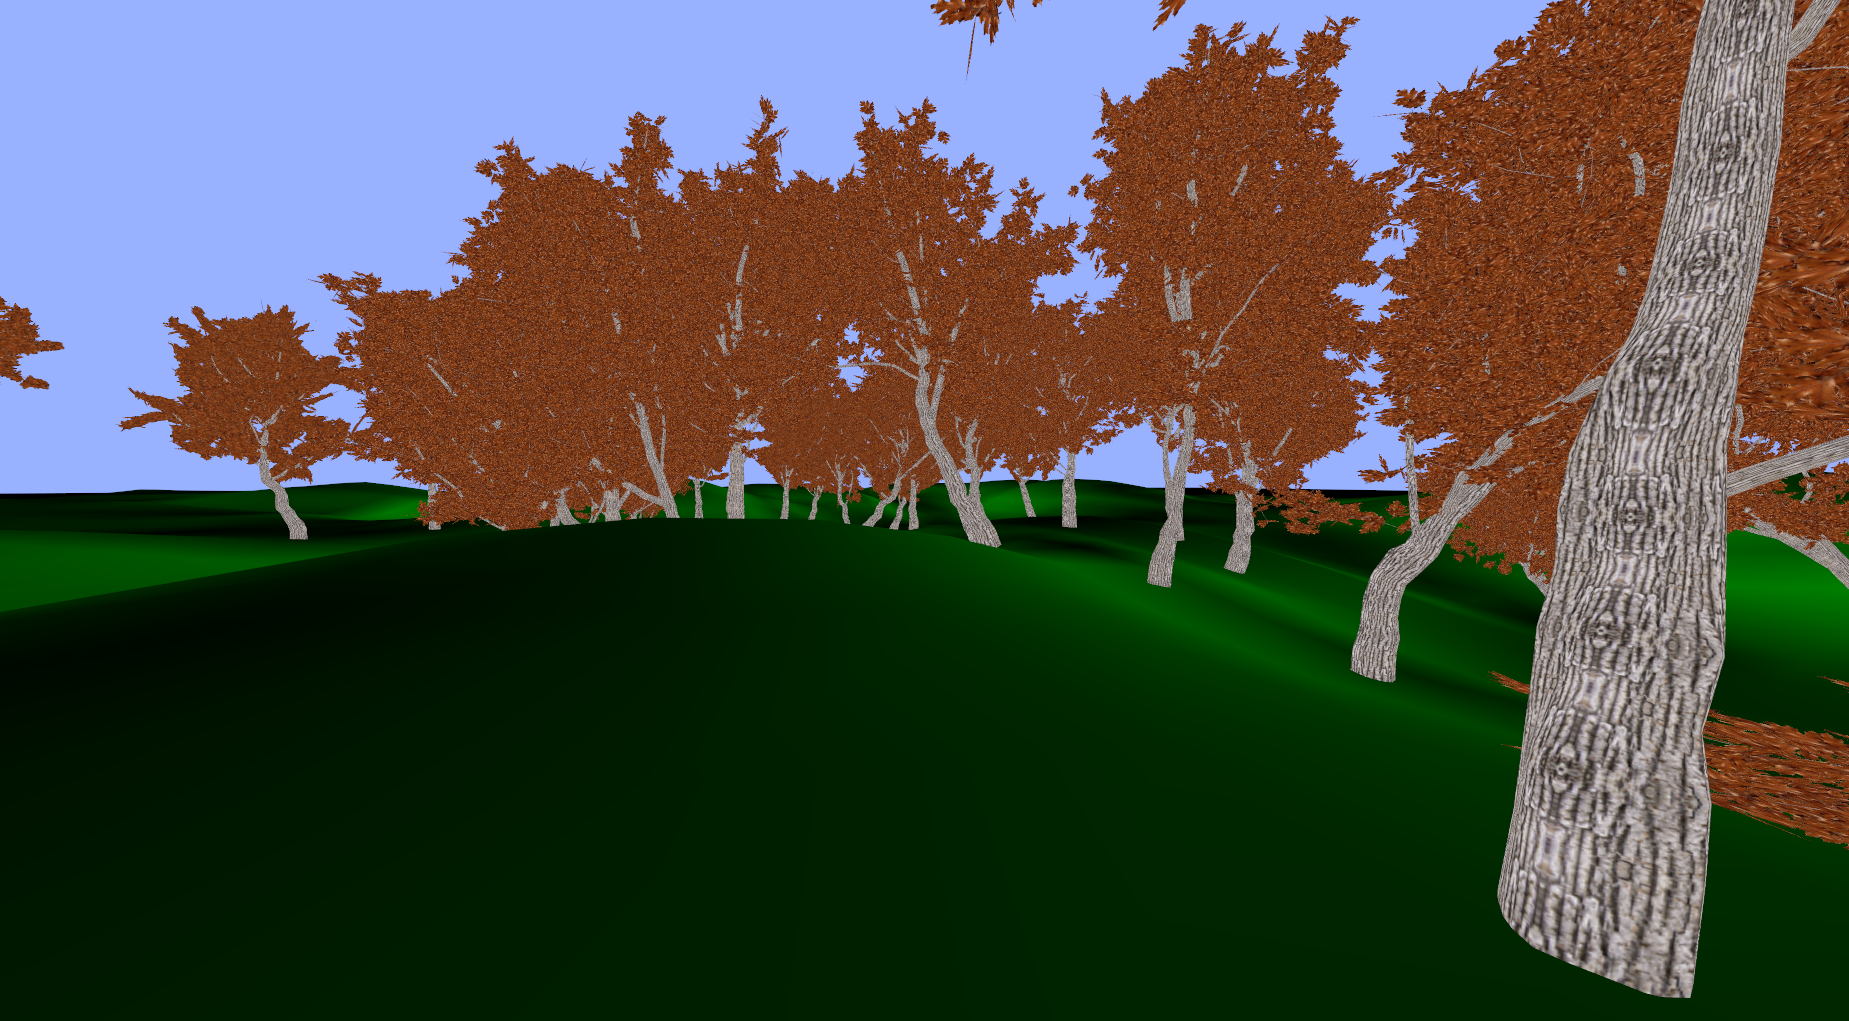
\includegraphics[scale=0.18]{clust.png}
\end{figure}
\end{frame}
\begin{frame}{Проблемы}

\textbf{Производительность:}\linebreak
Кластеризация 100 деревьев занимает 10-15 минут\linebreak
Cложность $O(n^2)$ от количества веток!\linebreak

\end{frame}
\begin{frame}{Синтетические деревья}
- Большинство деревьев растет в похожих условиях\linebreak
- Деревья одного типа похожи друг на друга\linebreak
- Кластеризация медленная\linebreak
- При росте числа деревьев количество кластеров тоже растет\linebreak\linebreak
\textbf{Решение}:\linebreak
Давайте собирать новые деревья из уже имеющихся частей!	\linebreak																
\end{frame}
\begin{frame}{Синтетические деревья}
1) Создаем относительно небольшую группу деревьев генератором\linebreak	
2) Проводим кластеризацию\linebreak	
3) Собираем статистику о параметрах кластеризованных деревьев\linebreak	
4) На основании нее синтезируем новые матрицы трансформации для существующих кластеров, которые формируют новые, "синтетические" деревья
\end{frame}
\begin{frame}{Сбор статистики}
\begin{figure}[hbtp]
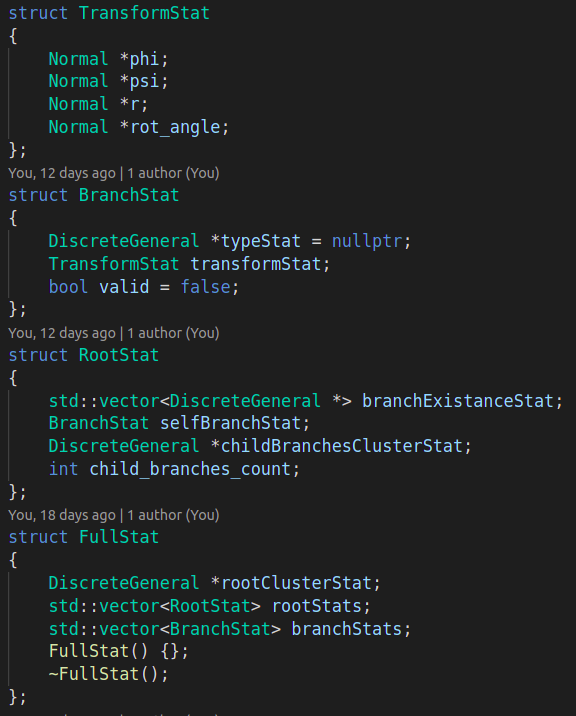
\includegraphics[scale=0.315]{stat.png}
\end{figure}
\end{frame}
\begin{frame}{Сбор статистики}
Геометрическое положение ветки задается положением ее конечной вершины в сферической СК с центром в начальной вершине и углом поворота вокруг своей оси\linebreak	
Считаем, что параметры эти распределены нормально, а параметры нормального распределения для каждого кластера(= типа) веток находим из статистики
\end{frame}
\begin{frame}{Создание синтетических деревьев}
- Выбираем место посадки по карте пригодности\linebreak	
- Выбираем тип ствола и его геометрические параметры\linebreak	
- Для каждой вершины ствола выбираем, сколько дочерних веток будет из него расти\linebreak	
- Делаем N попыток выбора дочерней ветки:\linebreak	
  Выбираем тип и геом. параметры\linebreak	
  Считаем суммарную освещенность ветки\linebreak	
- Выбираем вариант с наибольшим освещением и добавляем ее в воксельную карту освещения\linebreak	
- Формируем матрицы трансформации для ствола и веток\linebreak	
\end{frame}
\begin{frame}{Подготовка моделей}

- кластеризация деревьев целиком\linebreak
- создание импостеров\linebreak
- создание биллбордов\linebreak
- создание 3D-моделей\linebreak
\end{frame}
\begin{frame}{Level of Detail}
\begin{figure}[hbtp]
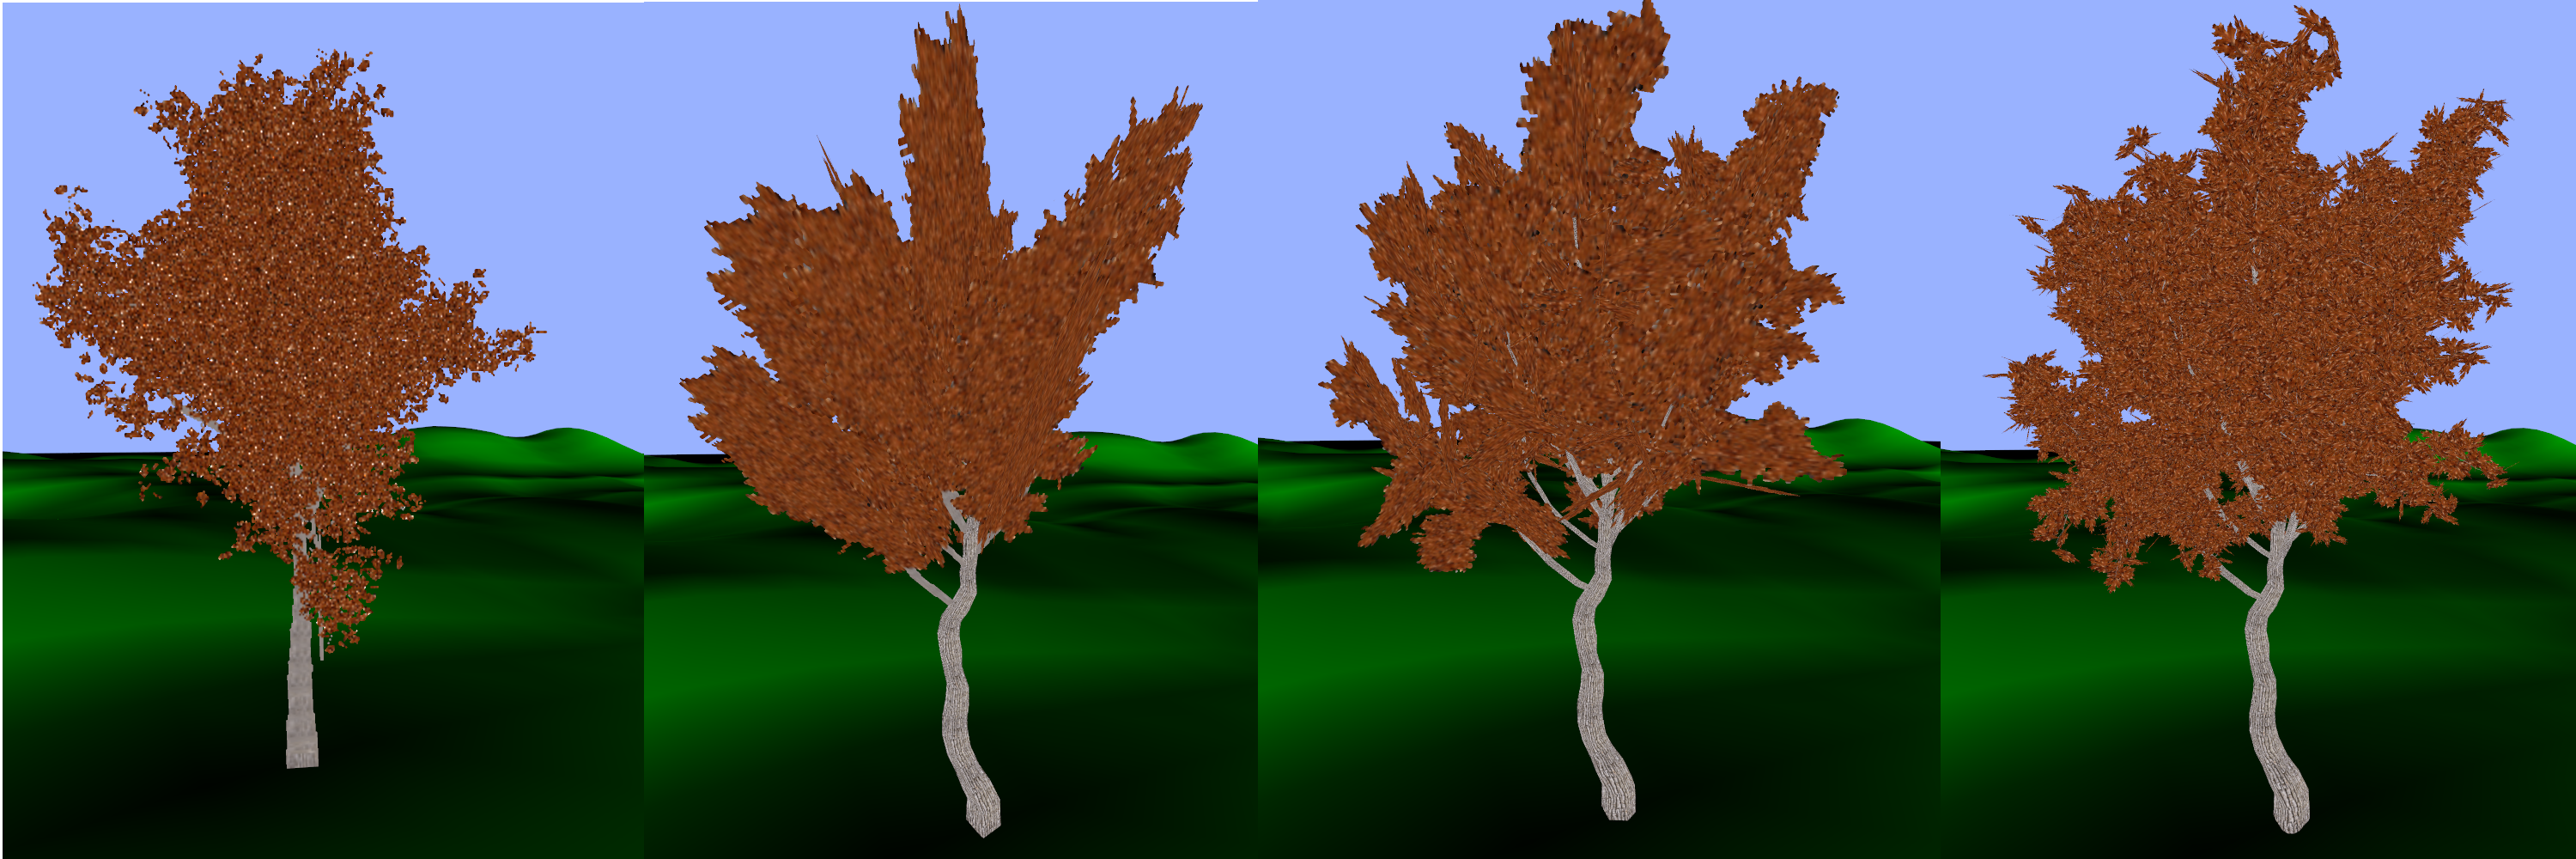
\includegraphics[scale=0.11]{lods.png}
\caption{4 уровня детализации}
\end{figure}
\end{frame}
\begin{frame}{Дальнейшее развитие}

- Эмпирическая метрика оценки визуального качества деревьев\linebreak
- Автоподбор параметров генератора\linebreak
- Сбор и использование глобальной статистики\linebreak
- Реализация кластеризации на GPU\linebreak
и многое другое...
\end{frame}
\begin{frame}{Конец}
Спасибо за внимание!
\end{frame}
\end{document}